\documentclass{article}

\usepackage{tikz} 

\usetikzlibrary{positioning} % Required for positioning of nodes
\usetikzlibrary{automata}    % Required for automata

\begin{document}

\begin{center}
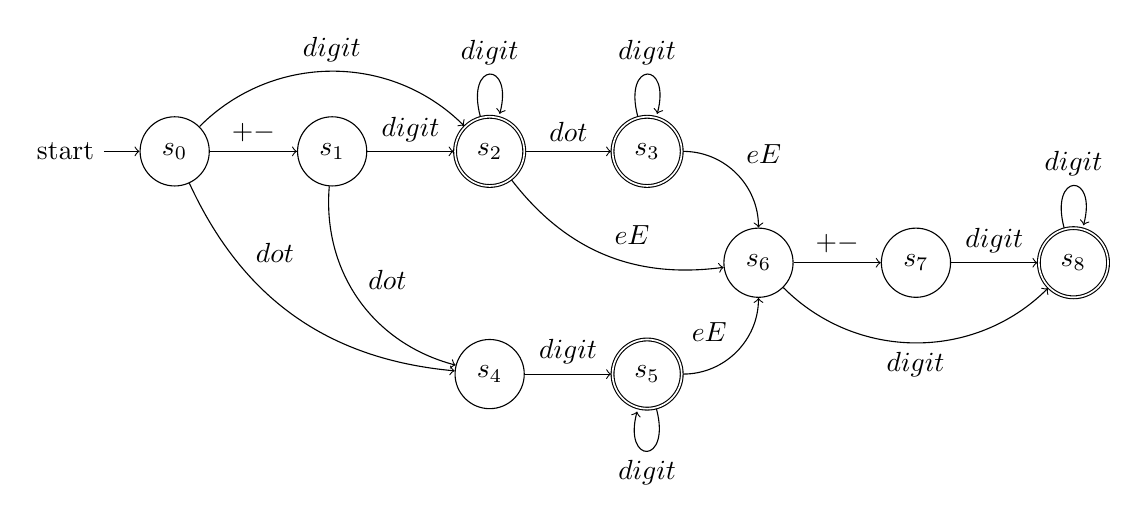
\begin{tikzpicture}[node distance=2cm, auto]
  % second automaton
  \node[state,initial]   (s0)                    {$s_0$};
  \node[state]           (s1) [right of=s0]      {$s_1$};
  \node[state,accepting] (s2) [right of=s1]      {$s_2$};
  \node[state,accepting] (s3) [right of=s2]      {$s_3$};
  \node[state]           (s6) [below right of=s3] {$s_6$};
  \node[state,accepting] (s5) [below left of=s6]      {$s_5$}; 
  \node[state]           (s4) [left of=s5]      {$s_4$};
  \node[state]           (s7) [right of=s6]     {$s_7$};
  \node[state,accepting] (s8) [right of=s7]     {$s_8$};
  \path[->] (s0) edge node {$+-$} (s1)
			     edge [bend left=45] node {$digit$} (s2) 
			     edge [bend right=30] node[pos=0.3] {$dot$} (s4) 
            (s1) edge node {$digit$} (s2)
	             edge [bend right=40] node {$dot$} (s4)
            (s2) edge [loop above] node {$digit$} ()
                 edge node {$dot$} (s3)
                 edge [bend right=30] node {$eE$} (s6)
            (s3) edge [loop above] node {$digit$} ()
                 edge [in=90,out=0] node {$eE$} (s6)
            (s4) edge node {$digit$} (s5)
            (s5) edge [loop below] node {$digit$} ()
                 edge [in=270,out=0] node {$eE$} (s6)
            (s6) edge node {$+-$} (s7)
                 edge [bend right=45] node[below] {$digit$} (s8)
            (s7) edge node {$digit$} (s8)
            (s8) edge [loop above] node {$digit$} ();
\end{tikzpicture}
\end{center}

\end{document}